\providecommand\classopts{}
\providecommand\geometryopts{}
\documentclass[a4paper,twoside\classopts]{memoir}
\usepackage[utf8]{inputenc}
\usepackage[pass\geometryopts]{geometry}
\usepackage[british]{babel}
\usepackage{csquotes}
\usepackage[T1]{fontenc}
\usepackage{charter}
\usepackage[bitstream-charter]{mathdesign}
\usepackage[final,babel]{microtype}
\usepackage{siunitx}
\usepackage{amsmath}
\usepackage{bm}
\usepackage{mathtools}
\usepackage{subcaption}
\usepackage{xpatch}
\usepackage[
  backend=biber,
  style=authoryear-comp,
  firstinits=true,
  doi=false,
  isbn=false,
  uniquename=init,
  uniquelist=minyear,
  labeldate=true,
  maxnames=2,
  hyperref=true]{biblatex}
\usepackage{minted}
\usepackage{booktabs}
\usepackage[hidelinks,pdfpagelayout=TwoPageRight]{hyperref}
\usepackage[final]{graphicx}
\usepackage{blindtext}
\usepackage{xcolor}

\addbibresource{journals.bib}
\addbibresource{dissertation.bib}

\makeatletter
\def\hrulefill{\leavevmode\leaders \hrule height \rulethickness \hfill\kern\z@}
\makeatletter

\title{Representation of Mountains in Atmospheric Models}
\author{James Shaw}
\date{August 2014}

\makeatletter
\AtBeginDocument{
  \hypersetup{
    pdftitle = {\@title},
    pdfauthor = {\@author}
  }
}
\makeatother
\OnehalfSpacing
\input{mysouthall}
\chapterstyle{mysouthall}
\blindmathtrue


\begin{document}
\newcommand{\TODO}[1]{\textcolor{purple}{TODO: \emph{#1}}}
\newcommand{\TODOsidenote}[1]{\marginpar{\footnotesize{\TODO{#1}}\vspace{0.3em}}}
\newcommand{\trans}[1]{{#1^\star}}
\newcommand{\surface}{h}
\newcommand{\shellcmd}[1]{\texttt{#1}}
\newcommand{\diffusioncoeff}{\mathcal{D}}
\newcommand{\exner}{\Pi}

\newcommand{\vect}{\bm}
\newcommand{\del}{\boldsymbol{\nabla}}

\begin{titlingpage}
\makeatletter
\begin{center}
\textsc{\Large University of Reading} \\[12pt]
{\Large Department of Meteorology} \\[16pt]
\includegraphics{uor-logo} \\[48pt]

\rule{\textwidth}{.4pt} \\[12pt]
{ \huge \bfseries \@title \\[16pt] } \rule{\textwidth}{.4pt} \\[54pt]
{\LARGE \@author}
\vfill
A dissertation submitted in partial fulfilment of the requirement for the degree of MSc Atmosphere Ocean and Climate \\[48pt]
{\Large \@date}
\end{center}
\makeatother
\end{titlingpage}


\frontmatter
\thispagestyle{plain}
\null\vfil
\begin{abstract}
\blindtext
\end{abstract}
\vfil

\cleardoublepage
\tableofcontents*

\mainmatter
\chapter{Introduction}

%- traditional NWP, hydrostatic models, used pressure coords, varied over time (steppeler2002)
%- current nonhydrostatic models have geometric vertical coords constant in time (steppeler2012)
%---------------------

Atmospheric flow over orography has significant effects on mesoscale weather, and even affects synoptic scale and global circulation \autocite{good2013}.

Current numerical weather prediction (NWP) models aim to forecast local weather.  Unlike their predecessors, these models operate on high resolution grids where the hydrostatic balance approximation is no longer valid and vertical acceleration cannot be neglected \autocite{steppeler2002}.

TODO: Vertical motion is important... orographically induced winds (steppeler2002), buoyancy effects.  Hence a vertical coordinate/grid that minimises numerical errors is desirable. TODO: distinguish between coordinates and grids (metric terms etc)

Terrain following coordinates are in widespread use in operational nonhydrostatic models.  In these vertical, geometric coordinate systems the terrain's influence decays with height: the bottommost layers follow the underlying surface closely while the uppermost layers are flat.  Such coordinates are attractive because cell sizes remain almost constant (Jebens 2011) and terrain following grids are simple to represent in a rectangular data structure (Lock2012),  However, as horizontal model resolution increases, steeper orographic gradients induce spurious winds due to numerical errors. \autocite{TODO}  TODO: elaborate on how these errors arise.  These are truncation errors?  Janjic 1989

TODO: what has been done to reduce these errors?
% Klemp 2011 presents this nicely
Basic terrain following (BTF) \autocite{galchen1975} 
\begin{align}
z = \left( z_t - h \right) \frac{\zeta}{z_t} + h = \zeta + \left( 1 - \frac{\zeta}{z_t} \right) h
\end{align}
where TODO define $z$, $z_t$, $\zeta$ and $h$ is the terrain height.

HTF (Arakawa and Lamb 1977) (Simmons and Burridge 1981)
SLEVE
STF (Klemp 2011)

The cut cell (or `shaved cell')  method is an alternative to terrain following coordinates.  Here, the surface terrain is intersected with a regular Cartesian grid such that cells are cut where they intersect with the ground.  TODO: disadvantage: boundary layer parameterisations (Zaengl 2012)

\chapter{Methodology}
\TODO{explain that we're using cartesian coords for everything.  See how Matt Jones justified this.}
\TODO{introduce the equation set and Hilary's discretisation}
\TODO{say something about how OpenFOAM always operates in 3D}

\section{Grid construction}
Two dimensional, regular cartesian grids were created using the OpenFOAM utility, \shellcmd{blockMesh}.  A custom utility was used to modify these orthogonal grids by adjusting the height of points to create terrain following grids.

\TODOsidenote{careful, you're changing tense a lot, James!}
At the time of writing, OpenFOAM does not directly support cartesian cut cell grids\footnote{An enhancement request was filed in 2013 to add support for cartesian cut cells to OpenFOAM, see \url{http://www.openfoam.org/mantisbt/view.php?id=1083}}.  Instead, the \shellcmd{snappyHexMesh} OpenFOAM utility was used to create a grid that approximates the cut cell method.  \TODO{describe how add2dMountain moves points up to the surface so that we retain small cells}.  A description of the surface is taken from any of the terrain following grids and the tool is used to intersect the surface with the grid.  The tool removes cells whose centres are below the surface.  The resulting grid is not strictly a cut cell mesh because, when \shellcmd{snappyHexMesh} moves points along the surface according to its heuristics, some points are moved horizontally.  It has not been possible to correct this issue for this project.
\TODOsidenote{Should I use codenames for the meshes, such as snapCol?  If not, what to say?  "Cut-cell style"?}

\begin{figure}
	\centerfloat
	\includegraphics[height=3in,angle=270]{mesh-snapCol-schaerExp-resting.eps}
	\caption{\TODO{cut cell grid}}
	\label{fig:method:cut-cell}
\end{figure}

\section{Discretisation of Euler equations}
\label{sec:method:discretisation}
The fully-compressible Euler equations used in the resting atmosphere test (section~\ref{sec:resting}) and gravity waves test (section~\ref{sec:gw}) are discretised following \textcite{weller-shahrokhi2014}.  \TODO{describe the important bits!}

\TODO{everything from this point is just notes right now}
\section{Meshes}

Test cases run on the following meshes:
\begin{description}
\item[snap]{snappyHexMesh applied to unmodified blockMesh}
\item[snapOrtho]{snappyHexMesh applied to blockMesh modified with add2dMountain.  Points nearest the surface were moved vertically to meet the surface.  See comparison in Figure~\ref{fig:snap-mesh-compare}.  I haven't run any tests against this mesh (yet) though.}
\end{description}

\begin{figure}
\includegraphics[width=\textwidth]{interim-results/cutCellWarpToSurfaceSchaerExp.png}
\caption{Comparison of snappyHexMesh on blockMesh versus snappyHexMesh after adjustment by add2dMountain.  The latter is more orthogonal.}
\label{fig:snap-mesh-compare}
\end{figure}

\chapter{Results}
\section{Advection}
Following \textcite{schaer2002}, a scalar tracer is transported above the orography by solving the advection equation for a prescribed horizontal wind.  \TODO{what does the test demonstrate?  that the effect of the grid dominates the numerical error}
The wind profile, terrain profile and initial tracer field are shown in Figure~\ref{fig:advection:initial}.

\subsection{Specification}
The domain is \SI{300}{\kilo\meter} wide and \SI{25}{\kilo\meter} high.  The terrain is wave-shaped, specified by the surface height $\surface$ such that
\begin{align}
	\surface(x) &= \cos^2 \left( \frac{\pi x}{\lambda} \right) \surface^\star
%
	\intertext{where}
%
	\surface^\star(x) &= \left\{ \begin{array}{l l}
		h_0 \cos^2 \left( \frac{\pi x}{2a} \right) & \quad \text{if $| x | < a$} \\
		0 & \quad \text{otherwise}
	\end{array} \right.
\end{align}
where $a = \SI{25}{\kilo\meter}$ is the mountain half-width, $h_0 = \SI{3}{\kilo\meter}$ is the maximum mountain height, and $\lambda = \SI{8}{\kilo\meter}$ is the wavelength.  On the SLEVE grid, the large-scale component $\surface_1$, as described in section~\ref{sec:theory:sleve}, is given by
\begin{align}
	\surface_1(x) &= \frac{1}{2}\surface^\star(x)
\end{align}
and $s_1 = \SI{15}{\kilo\meter}$ is the large scale height, and $s_2 = \SI{2.5}{\kilo\meter}$ is the small scale height.  The optimisation of SLEVE by \textcite{leuenberger2010} is not used, so the exponent $n = 1$.

For comparison, the same tests were performed with no orography, such that $\surface = \SI{0}{\kilo\meter}$ everywhere.

The wind is entirely horizontal and is prescribed as
\begin{align}
	u(z) = u_0 \left\{ \begin{array}{l l}
		1 & \quad \text{if $z \geq z_2$} \\
		\sin^2 \left( \frac{\pi}{2} \frac{z - z_1}{z_2 - z_1} \right) & \quad \text{if $z_1 < z < z_2$} \\
		0 & \quad \text{otherwise}
	\end{array} \right.	
\end{align}
where $u_0 = \SI{10}{\meter\per\second}$, $z_1 = \SI{4}{\kilo\meter}$ and $z_2 = \SI{5}{\kilo\meter}$.
This results in a constant wind aloft, and zero flow at \SI{4}{\kilo\meter} and below.
A tracer $\varphi$ is positioned upstream above the height of the terrain.  It has the shape
\begin{align}
	\varphi(x, z) &= \varphi_0 \left\{ \begin{array}{l l}
		\cos^2 \left( \frac{\pi r}{2} \right) & \quad \text{if $r \leq 1$} \\
		0 & \quad \text{otherwise}
	\end{array} \right.
%
\intertext{having radius $r$ given by}
%
	r &= \sqrt{
		\left( \frac{x - x_0}{A_x} \right)^2 + 
		\left( \frac{z - z_0}{A_z} \right)^2
	}
\end{align}
where $A_x = \SI{25}{\kilo\meter}$, $A_z = \SI{3}{\kilo\meter}$ are the horizontal and vertical half-widths respectively, and $\varphi_0 = 1$ is the maximum magnitude of the anomaly.  At $t = \SI{0}{\second}$, the anomaly is centred at $(x_0, z_0) = (\SI{-50}{\kilo\meter}, \SI{9}{\kilo\meter})$ so that the anomaly is upwind of the mountain and well above the maximum terrain height of \SI{3}{\kilo\meter}.  Analytic solutions can be found by adjusting the anomaly centre such that $x_0 = ut$.

\begin{figure}
	\centerfloat
	\input{advection-initial-plot}
	\caption{Vertical cross section of the two-dimensional advection test showing the horizontal wind profile, surface terrain profile and scalar tracer field at $t = \SI{0}{\second}$ on a $\SI{300}{\kilo\meter} \times \SI{25}{\kilo\meter}$ domain.  Adapted from \textcite{schaer2002}.}
	\label{fig:advection:initial}
\end{figure}

\subsection{Discretisation}
The OpenFOAM solver \shellcmd{scalarTransportFoam} was used to implicitly solve the advection-diffusion equation in flux form
\begin{align}
	\frac{\partial \varphi}{\partial t} + \del \cdot \left( \vect{u} \varphi \right) - \laplace \left( \diffusioncoeff \varphi \right) = 0 \label{eq:advection:continuous}
\end{align}
Diffusion was turned off by setting the diffusion coefficient $\diffusioncoeff$ to be zero.

The time derivative ($\partial \varphi / \partial t$) is solved implicitly using a backward-in-time, second order accurate scheme defined as \autocite{openfoam-progguide}
\begin{align}
	\frac{\partial}{\partial t} \int_V \varphi \diff V = \frac{
		3 \left( \varphi V \right)^{(n)} - 
		4 \left( \varphi V \right)^{(n-1)} + 
		\left( \varphi V \right)^{(n-2)}
	}{2 \Delta t}
\end{align}

Spatial discretisation follows the finite volume method described in section~\ref{sec:theory:fv}.
Two spatial interpolations were tested.  First, the van Leer scheme which blends two schemes to maximise boundedness and accuracy.  It combines a centred difference scheme that is second-order accurate and unbounded with an upwind scheme that is first-order accurate and bounded.  The interpolated value $\varphi_F$ is calculated as a weighted average of the interpolated values from the two schemes, $\varphi_{F,\mathrm{upwind}}$ and $\varphi_{F,\mathrm{centred}}$, such that
\begin{align}
	\varphi_F &= \left( 1 - \gamma \right) \varphi_{F,\mathrm{upwind}} + \gamma \varphi_{F,\mathrm{centred}}
\end{align}
The van Leer scheme defines the blending coefficient $\gamma$ as a function of the ratio $r$ between the upwind and local gradient of $\varphi$.  The blending coefficient is specified as \autocite{leveque2002}
\begin{align}
\gamma(r) &= \frac{r + |r|}{1 + |r|}
%
\intertext{and the gradient ratio is specified by \textcite{weller2012} as}
%
	r &= \frac{2 \left( \vect{x_d} - \vect{x_u} \right) \cdot \del_u \phi}{\varphi_d - \varphi_u} - 1
\end{align}
where $\vect{x}$ is the position vector of the cell centre and subscripts $u$ and $d$ denote upwind and downwind cells respectively.

\TODO{Second, a TVD limited version of upwind-biased cubic scheme...  I might not have time to discuss this, but it does offer a modest improvement at the expense of increased computation}

The domain is discretised onto a grid having $300 \times 50$ cells such that $\Delta x = \SI{1}{\kilo\meter}$ and $\Delta \trans{z} = \SI{500}{\meter}$.  Unlike \textcite{schaer2002} which used periodic lateral boundaries, we use zero gradient boundary conditions for all boundaries.
Tests are integrated forward in time for \SI{10000}{\second} with a timestep $\Delta t = \SI{25}{\second}$.  \TODOsidenote{we never looked at courant numbers, but Schaer talks about horiz/vertical Co numbers}

\subsection{Results}
\begin{figure}
	\captionsetup[subfigure]{position=b}
	\centering
	\subcaptionbox{BTF \label{fig:advection:vanLeer:btf}}[0.49\textwidth]{\input{advection-btf-schaerCos-vanLeer-contour-plot}}
	\hfill
	\subcaptionbox{BTF \label{fig:advection:schaer:btf}}[0.49\textwidth]{\vspace{0.43in}\includegraphics[height=1.2in]{img/schaer-btf-centred.png}}
\\
	\subcaptionbox{SLEVE \label{fig:advection:vanLeer:sleve}}[0.49\textwidth]{\input{advection-sleve-schaerCos-vanLeer-contour-plot}}
	\hfill
	\subcaptionbox{SLEVE \label{fig:advection:schaer:sleve}}[0.49\textwidth]{\vspace{0.43in}\includegraphics[height=1.2in]{img/schaer-sleve-centred.png}}
\\
	\subcaptionbox{Cut cell \label{fig:advection:vanLeer:cutCell}}[0.49\textwidth]{\input{advection-snapCol-schaerCos-vanLeer-contour-plot}}
	\hfill
	\subcaptionbox{Analytic solution on a regular grid}[0.49\textwidth]{\input{advection-noOrography-analytic-contour-plot}}
%
	\caption{\TODO{van Leer advection compared with schaer -- centred scheme.  Contour intervals every 0.1}}
	\label{fig:advection:vanLeer}
\end{figure}

Results of advection using the van Leer scheme are presented in Figure~\ref{fig:advection:vanLeer}.  On the BTF grid, the tracer suffers from distortion over the mountain and some artefacts just above the mountain remain as the tracer moves over it.  Compared with the results from \textcite{schaer2002}, the tracer retains more of its shape but suffers from far more numerical diffusion by the end of the simulation, as evidenced by the missing contours in the tracer centre.  \TODO{would it be worth looking at variance at t=10000s to quantify the diffusion?}

Results on the SLEVE grid are much closer to the analytic solution on a regular grid.  The tracer retains its shape throughout the simulation and does not suffer from any noticeable distortion.  However, the widening contours indicate some numerical diffusion is still present which, again, was not found in the results of \textcite{schaer2002}.

Since the cut cell grid is entirely regular away from the surface, it is unsurprising that the results are the same as advection on a regular grid (not shown).  This result agrees with that found by \textcite{good2013}.

\TODO{we could try plotting diffs as done by schaer2002, too}

\TODO{now discuss tvdLimitedCubicUpwindCPCFit}
\TODO{tvdLimitedCubicUpwindCPCFit slightly better than vanLeer, but much more computationally expensive}

Error norms were calculated at $t = \SI{10000}{\second}$ by comparing with the analytic solution.  The $\ell^2$ error norm is defined as
\begin{align}
\ell^2 = \sqrt{\frac{\sum \left( \varphi - \varphi_T \right)^2 \cdot V}{\sum V}}
\end{align}
where $\varphi$ is the numerical tracer value, $\varphi_T$ is the analytical value and $V$ is the cell volume.  Because the test is two dimensional, the cell volume is equivalent to the cell area.  The resulting errors are summarised in table~\ref{tab:advection:errors}.  \TODO{what do they tell us?}

\begin{table}
\centering
\begin{tabular}{ r @{\hspace{2em}} l l}
\toprule
		&	van Leer	& Cubic upwind \\ \midrule
BTF		& \input{openfoam/cases/advection/btf/schaerCos/vanLeer/l2error.txt}		& \TODO{0} \\
SLEVE		& \input{openfoam/cases/advection/sleve/schaerCos/vanLeer/l2error.txt}		& \TODO{0} \\
Cut cell	& \input{openfoam/cases/advection/snapCol/schaerCos/vanLeer/l2error.txt}	& \TODO{0} \\ \bottomrule
\end{tabular}

\caption{$\ell^2$ error norms for the advection test at $t = \SI{10000}{\second}$}
\label{tab:advection:errors}
\end{table}


\section{Resting atmosphere}
Compared meshes, and dp/dx versus H operator.

\begin{itemize}
\item Max vertical velocities compared in Figure~\ref{fig:rest:w}
\item Energy change compared (see Figure~\ref{fig:rest:energy-tf}, \ref{fig:rest:energy-cut-cell})
\item H operator always outperforms dp/dx
\item All cut-cell style meshes outperform TF meshes in this test in terms of $w$ and energy change
\end{itemize}
Some issues were found:
\begin{itemize}
\item noOrography should have zero $w$, but actually has \SI{1e-10}{\meter\per\second}.  Hilary says this is due to loss of precision when reading initial fields (should be in discrete hydrostatic balance).
\item Computational oscillation in BTF H operator after about 4 hours (Figure~\ref{fig:rest:energy-tf})
\end{itemize}

\begin{figure}
\includegraphics[width=\textwidth]{interim-results/verticalVelocityPlotSnappyHexMesh.png}
\caption{Max vertical velocities (note log scale on y axis)}
\label{fig:rest:w}
\end{figure}

\begin{figure}
BTF H
\includegraphics[width=\textwidth]{interim-results/restingBtfHEnergy.png}
SLEVE
\includegraphics[width=\textwidth]{interim-results/restingSleveEnergy.png}
\caption{Energy changes (TF)}
\label{fig:rest:energy-tf}
\end{figure}

\begin{figure}
SnapCol
\includegraphics[width=\textwidth]{interim-results/restingSnapColEnergy.png}
Snap
\includegraphics[width=\textwidth]{interim-results/restingSnapEnergy.png}
\caption{Energy changes (cut-cell style)}
\label{fig:rest:energy-cut-cell}
\end{figure}

\section{Gravity waves}
\label{sec:gw}

\TODO{introduce the test, justify its purpose}
\TODO{it might be nice to have some theory on gravity waves (e.g. how theta/w anomalies are created and their positions in space), then compare model results with theory}

\subsection{Specification}
Following \textcite{melvin2010}, the domain is \SI{300}{\kilo\meter} wide and \SI{30}{\kilo\meter} high.  The mountain profile has the same form as equation~\ref{eqn:resting:mountain} but with a lower maximum height of $\surface_0 = \SI{250}{\meter}$.  As in the resting atmosphere test, $a = \SI{5}{\kilo\meter}$ is the mountain half-width and $\lambda = \SI{4}{\kilo\meter}$ is the wavelength.  On the optimised SLEVE grid, $s_1 = \SI{5}{\kilo\meter}$ is the large scale height, $s_2 = \SI{2}{\kilo\meter}$ is the small scale height and the optimal exponent value $n = 1.35$ as in the previous test\TODOsidenote{where did these SLEVE parameters come from?}.

The initial thermodynamic conditions have a surface temperature of $\theta_0 = \SI{288}{\kelvin}$ and constant stability with $N = \SI{0.01}{\per\second}$ everywhere.  A constant horizontal wind $u = \SI{10}{\meter\per\second}$ is prescribed at the inlet boundary.

\subsection{Discretisation}
The test uses the discretisation of the Euler equations described in section~\ref{sec:method:discretisation}.  The domain is discretised on a grid having $600 \times 100$ cells such that $\Delta x = \SI{0.5}{\kilo\meter}$ and $\Delta z = \SI{300}{\meter}$.  Sponge layers are added to the upper \SI{10}{\kilo\meter} and leftmost \SI{10}{\kilo\meter} at the inlet boundary to damp the reflection of waves.
The term $\mu \rho \vect{u}$ is subtracted from the momentum equation (equation~\ref{eqn:method:momentum}) where the damping function $\mu$ is adapted from \textcite{melvin2010} such that
\begin{align}
	\mu(x, z) &= \mu_\mathrm{upper} + \mu_\mathrm{inlet} \\
	\mu_\mathrm{upper}(z) &= \begin{cases}
		\overline{\mu} \sin^2 \left( \frac{\pi}{2} \frac{z - z_B}{H - z_B} \right) & \text{if } z \geq z_B \\
		0 & \text{otherwise} \\
	\end{cases} \\
	\mu_\mathrm{inlet}(x) &= \begin{cases}
		\overline{\mu} \sin^2 \left( \frac{\pi}{2} \frac{x_I - x}{x_I - x_0} \right) & \text{if } x < x_I \\
		0 & \text{otherwise}
	\end{cases}
\end{align}
where $\overline{\mu} = 1.2$ is the damping coefficient, $z_B = \SI{20}{\kilo\meter}$ is the bottom of the sponge layer, $H = \SI{30}{\kilo\meter}$ is the top of the domain, $x_0 = \SI{-150}{\kilo\meter}$ is the leftmost limit of the domain and $x_I = \SI{-140}{\kilo\meter}$ is the rightmost extent of the inlet sponge layer.  Note that, while the domain itself is \SI{30}{\kilo\meter} in height, for the purposes of generating of BTF and SLEVE grids, the domain height is set to \SI{20}{\kilo\meter} because the sponge layer occupies the uppermost \SI{10}{\kilo\meter}.

No slip conditions are imposed on the top and bottom boundaries and the outlet is zero gradient.  For Exner, hydrostatic balance is prescribed on all boundaries.  The simulation is integrated forward by 5 hours with a timestep $\Delta t = \SI{8}{\second}$.

\subsection{Results}


\begin{figure}
	\captionsetup[subfigure]{position=b}
	\centering
	\subcaptionbox{BTF \label{fig:gw:w:btf}}[0.48\textwidth]{\includegraphics[height=2.6in,angle=270]{data/gravityWaves-btf-schaerExp-h/18000/w.eps}}
	\hfill
	\subcaptionbox{Mass-conserving semi-implicit semi-Lagrangian solution from \textcite{melvin2010} \label{fig:gw:w:melvin}}[0.48\textwidth]{\includegraphics[height=2in]{img/melvin-7a.png}} \\
	\subcaptionbox{SLEVE \label{fig:gw:w:sleve}}[0.48\textwidth]{\includegraphics[height=2.6in,angle=270]{data/gravityWaves-sleve-schaerExp-h/18000/w.eps}}
	\hfill
	\subcaptionbox{SLEVE \label{fig:gw:thetaDiff:sleve}}[0.48\textwidth]{\includegraphics[height=2.6in,angle=270]{data/gravityWaves-sleve-schaerExp-h/18000/thetaDiff.eps}} \\
	\subcaptionbox{SnapCol \label{fig:gw:w:snapCol}}[0.48\textwidth]{\includegraphics[height=2.6in,angle=270]{data/gravityWaves-snapCol-schaerExp-h/18000/w.eps}}
	\hfill
	\subcaptionbox{SnapCol \label{fig:gw:thetaDiff:snapCol}}[0.48\textwidth]{\includegraphics[height=2.6in,angle=270]{data/gravityWaves-snapCol-schaerExp-h/18000/thetaDiff.eps} \TODO{include legend}}
	\caption{\TODO{w contours, every \SI{5e-2}{\meter\per\second}.  $t = \SI{18000}{\second}$ Compared with fig 7a from \textcite{melvin2010}.}}
	\label{fig:gw:w}
\end{figure}

\begin{figure}
	\captionsetup[subfigure]{position=b}
	\centering
	\subcaptionbox{SLEVE \label{fig:gw:thetaDiffZoom:sleve}}[\textwidth]{\includegraphics[width=1.6in,angle=270]{data/gravityWaves-sleve-schaerExp-h/18000/nonlinearMomentumZoom.eps}} \\
	\subcaptionbox{SnapCol \label{fig:gw:thetaDiffZoom:snapCol}}[\textwidth]{\includegraphics[width=1.6in,angle=270]{data/gravityWaves-snapCol-schaerExp-h/18000/nonlinearMomentumZoom.eps}}
	\caption{\TODO{Theta anomalies (zoomed in).  I've superimposed nonlinear momentum vectors but I'm not sure how/if I can discuss them.}}
	\label{fig:gw:thetaDiffZoom}
\end{figure}

Comparing vertical velocity contours between BTF and SLEVE show few visible differences (figures~\ref{fig:gw:w:btf}, \subcaptionref{fig:gw:w:sleve}).  Since the same model was used, these results match those from \textcite{weller-shahrokhi2014}.  Vertical velocities on the SnapCol grid are similar to the terrain following results (figure~\ref{fig:gw:w:snapCol}).  All three results are in agreement with a semi-implicit, semi-Lagrangian simulation from \textcite{melvin2010} (see figure~\ref{fig:gw:w:melvin}).

Theta anomalies are similar on all grids, having a similar shape to vertical velocity contours, but phase shifted by \ang{180} (SLEVE grid figure~\ref{fig:gw:thetaDiff:sleve}, SnapCol grid figure~\ref{fig:gw:thetaDiff:snapCol}, BTF grid not shown). 
Examining more closely the potential temperature anomaly on the SnapCol grid, in the lee of the mountain the bottommost layer is anomalously warm and the layer above it is anomalously cold (figure~\ref{fig:gw:thetaDiffZoom:snapCol}).  Potential temperature increases with height because the simulated atmosphere is stable, so these anomalies serve to reduce the stability near the ground.  The anomalies are not sufficiently large to destabilise the atmosphere, however.   Therefore, vertical motion is not expected, and was not observed, near the ground on the lee side.   Whilst turbulent motion does cause such thermal mixing in the real atmosphere, there is no viscosity in the model equations, so the thermal anomalies should not be present.  The feature is not present on the SLEVE grid (figure~\ref{fig:gw:thetaDiffZoom:sleve}) or BTF grid (not shown).

\begin{figure}
	\subcaptionbox{SLEVE}[\textwidth]{\includegraphics[width=1.6in,angle=270]{data/gravityWaves-sleve-schaerExp-h/18000/UfZoom.eps}} \\
	\subcaptionbox{SnapCol}[\textwidth]{\TODO{}} \\
	\caption{\TODO{SLEVE and SnapCol flows}}
	\label{fig:gw:flow}
\end{figure}

\hrule

\begin{itemize}
\item Vertical mixing at ground in lee of orography seen in results for snapCol and snap meshes.  This occurs in the lowest two rows of the mesh: lower layer $\theta$ is warmer, next layer above is cooler.  Feature is visible after t=3600s (Figure~\ref{fig:gw:mixing-3600s}), becomes more pronounced by t=18000s (Figure~\ref{fig:gw:mixing-18000s}).
\end{itemize}

\subsection{Investigation of vertical mixing}
Initially suspected mixing was due to computation mode of Lorenz vertical staggering but now it seems not (or maybe it does! we're not quite sure!)
\begin{itemize}
	\item plot UfDiff as a vector field doesn't seem to show any velocity anomalies in BTF or snalCol (Figure~\ref{fig:gw:ufdiff})
	\item plot of $\theta$ field shows that mixing is not strong enough to overcome stratification (Figure~\ref{fig:gw:theta})
	\item doubling mountain height causes mixing to appear in BTF case, and increases to three rows of mixing in SnapCol (Figure~\ref{fig:gw:double-height})
	\item halving $\Delta z$ also causes BTF mixing but less severe, also three rows of mixing in SnapCol (not shown)
	\item the results for dp/dx show mixing in BTF, and increased mixing in SnapCol (not shown)
\end{itemize}


This suggests irreversible thermodynamic mixing (caused by numerical errors).  In reality, viscous effects would cause such mixing, but our equation set has no viscosity so there should be no mixing.

By isolating the nonlinear advection term in the momentum equations ($\del \rho \vect{u} \vect{u}$) we can see the different in flows between BTF and SnapCol meshes (Figure~\ref{fig:gw:nonlinear-advection}).  Looking at $U_f$ we can see larger velocities in small cells near mountain peaks, but otherwise flow fields are qualitatively in good agreement.

Noticing that $U_f$ follows the BTF mesh but does not follow the SnapCol mesh, we suspect that the thermal mixing may be caused by numerical diffusion (as we same with horizontal tracer advection).  This time, however, the flow is not horizontal, so it is SnapCol that has more diffusion.

\subsection{Courant number}

\begin{itemize}
	\item Mean Courant numbers for cut-cell meshes and SLEVE are lower than BTF.  This could be because cells are relatively smaller aloft.
	\item Surprisingly, mean Courant number is slightly higher for snap mesh which has no small cells (Figure~\ref{fig:gw:courant}).
	\item SLEVE and BTF have the lowest max Co numbers, snap mesh significantly higher.  Since snap mesh does not have small cells, does this imply that snap mesh has higher winds?
\end{itemize}

Hilary mentioned that the reason that small cells aren't too much of a problem is that the small face is vertically oriented and has the majority of the flow fluxing through it.

\begin{align}
	\mathrm{Co} &= \frac{\Delta t}{2 V \rho} \sum{U}
	\intertext{where $U = \rho \vect{u} \cdot \vect{S}$ (ish.  see Eqn 6 in W\&S2014).  Given large near-horizontal surface $S_1$ and adjoining small vertical surface $S_2$}
	&= \frac{\Delta t}{2 S_1 S_2} \left( \vect{u} \cdot S_1 + \vect{u} \cdot S_2 \right)
	\intertext{which, when $S_2$ is sufficiently small}
	&\approx \frac{\Delta t}{2 S_1} \left( \vect{u} \cdot S_1 \right)
\end{align}
Hence, the Courant number is less affected by small cells with near-horizontal flow.

\begin{itemize}
	\item We can try increasing $\Delta t$ until SnapCol becomes unstable ($\mathrm{Co} > 1$), and compare results with TF meshes (and possibly Snap/SnapOrtho meshes) with the same timestep.  This will show that small cells are a problem.
	\item We could even try a sinking bubble test where the momentum will be fluxing through the large, almost-horizontally oriented face along the terrain surface
\end{itemize}

\begin{figure}
	\includegraphics[width=\textwidth]{interim-results/gravityWavesCourants.png}
	\caption{Courant number for gravityWaves}
	\label{fig:gw:courant}
\end{figure}

\subsection{Energy}
\begin{itemize}
	\item Cut cell meshes are worse than TF meshes.  Snap loses internal energy much quicker than other meshes; i.e. it gets colder. (Figure~\ref{fig:gw:energy})
\end{itemize}

\begin{figure}
	\includegraphics[width=\textwidth]{interim-results/gravityWavesEnergy.png}
	\caption{Energy changes}
	\label{fig:gw:energy}
\end{figure}

Looking at max Courant number for SLEVE, and energy loss graphs for all meshes, we see a change of behaviour at t=10000s (about 2.8 hours).  This might be related to gravity waves reflecting off the inlet or outlet boundary.  Changing the wind speed would let us investigate further.



\backmatter
\printbibliography

\end{document}
